\documentclass[10pt,landscape,a4paper]{article}
\usepackage[utf8]{inputenc}
\usepackage[nosf]{kpfonts}
\usepackage[t1]{sourcesanspro}

% For the multiple columns in the cheat sheet
\usepackage{multicol}

% Set the margins of the paper
\usepackage[margin=1mm]{geometry}

% To use colours
\usepackage{xcolor}

% To typeset small fonts
\usepackage{microtype}

% To have easier typesetting of units
\usepackage{siunitx}

% To include graphics
\usepackage{graphicx}

\graphicspath{ {./images/} }

\let\bar\overline

\definecolor{myblue}{cmyk}{1,.72,0,.38}

\everymath\expandafter{\the\everymath \color{myblue}}
\everydisplay\expandafter{\the\everydisplay \color{myblue}}

\renewcommand{\baselinestretch}{.8}
\pagestyle{empty}

\makeatletter
\renewcommand{\section}{\@startsection{section}{1}{0mm}%
  {.2ex}%
  {.2ex}%x
  {\color{myblue}\sffamily\small\bfseries}}
\renewcommand{\subsection}{\@startsection{subsection}{1}{0mm}%
  {.2ex}%
  {.2ex}%x
  {\sffamily\bfseries}}


\makeatother
\setlength{\parindent}{0pt}

\begin{document}
\small
\begin{multicols*}{5}
  \raggedcolumns


  \section{Fourier Series}

  Amplitude linearity: \\
  \(V_{out} (t) - V_{out} (0) = \alpha (V_{in} (t) - V_{in} (0))\)

  Fundamental frequency: \\
  \(\omega_0 = \frac{2\pi}{T} = 2\pi f_0\)

  General form: \\
  \(F(t) = C_0 + \sum_{n = 1}^{\infty} A_n \cos (n \omega_0 t) + \sum_{n = 1}^{\infty} B_n \sin (n \omega_0 t)\) \\
  \(C_0 = \frac{1}{T} \int_0^T f(t) \, dt = \frac{A_0}{2}\) \\
  \(A_n = \frac{2}{T} \int_0^T f(t) \cos(n \omega_0 t) \, dt\) \\
  \(B_n = \frac{2}{T} \int_0^T f(t) \sin(n \omega_0 t) \, dt\)

  Complex form (standard form): \\
  \(F(t) = \sum_{n = - \infty}^{\infty} D_n e^{jn \omega_0 t} \, dt\) \\
  \(D_n = \frac{1}{T} \int_{- \frac{T}{2}}^{\frac{T}{2}} f(t) e^{-jn \omega_0 t}\) \\
  \(D_n = \frac{A_n - j B_n}{2}\)

  Cosine form: \\
  \(C_n = \sqrt{A_n^2 + B_n^2}\) \\
  \(\phi_n = - \arctan \left(\frac{B_n}{A_n} \right)\) \\
  \(F(t) = C_0 + \sum_{n = 1}^{\infty} C_n \cos(n \omega_0 t + \phi_n)\)

  Sine form: \\
  \(C_n = \sqrt{A_n^2 + B_n^2}\) \\
  \(\phi_n^* = \arctan \left(\frac{A_n}{B_n} \right)\) \\
  \(F(t) = C_0 + \sum_{n = 1}^{\infty} C_n \sin(n \omega_0 t + \phi_n^*)\)

  Evenness: \\
  \(f(t) g(t)\) and \(\frac{f(t)}{g(t)}\) are even only if both \(f(t)\) and \(g(t)\) are either even or odd

  Even function: \\
  \(B_n = 0\) \\
  \(A_n = \frac{4}{T} \int_0^{\frac{T}{2}} f(t) \cos(n \omega_0 t) \, dt\) \\
  \(C_0 = \frac{1}{T} \int_{-\frac{T}{2}}^{\frac{T}{2}} f(t) \, dt\)

  Odd function: \\
  \(A_n = 0\) \\
  \(C_0 = 0\) \\
  \(B_n = \frac{4}{T} \int_0^{\frac{T}{2}} f(t) \sin(n \omega_0 t) \, dt\)

  \section{Linear systems}

  Linear systems: \\
  \(\sum_{n = 0}^N A_n \frac{d^n X_{out}}{dt^n} = \sum_{m = 0}^M B_m \frac{d^m X_{in}}{dt^m}\)

  Homogeneous equation: \\
  \(\sum_{n = 0}^N A_n \frac{d^n X_{out}}{dt^t} = 0\)

  \subsection{Zero-order system}
  \(A_0 X_{out} = B_0 X_{in}\) \\
  \(X_{out} = KX_{in}\)

  \subsection{First-order system}

  Differential equations: \\
  \(A_1 \frac{d X_{out}}{dt} + A_0 X_{out} = B_0 X_{in}\) \\
  \(\tau \frac{d X_{out}}{dt} + X_{out} = K X_{in}\)

  General solution: \\
  \(x(t) = (x_0 - x_{\infty}) e^{-\frac{t}{\tau}} + x_{\infty}\)

  \subsection{Second-order system}

  Differential equation: \\
  \(A_2 \frac{d^2 X_{out}}{dt^2} + A_1 \frac{d X_{out}}{dt} + A_0 X_{out} = B_0 X_{in}\)

  Dynamic equation: \\
  \(F = m \ddot{x} + b \dot{x} + kx\)

  Frequency response \(\left(\frac{X}{F} \right)\): \\
  \(\frac{X}{F} = \frac{k^{-1}}{- \frac{\omega^2}{\omega_0^2} + \frac{j \omega}{Q \omega_0} + 1}\)

  Resonance: \\
  \(\omega_0^2 = \omega_n^2 = \frac{k}{m} = \frac{k}{I}\)

  Damping ratio: \\
  \(\zeta = \frac{b}{b_c} = \frac{b}{2 \sqrt{mk}}\)

  Mechanical \(Q\): \\
  \(Q^2 = \frac{km}{b}, \text{ when } Q = 0.5,\) the system is critically damped

  \subsection{Characteristic equation}

  Equation: \\
  \(\sum_{n = 0}^N A_n s^n = 0\)

  Primary (\(N = 1\)): \\
  \(A_1 s + A_0 = 0\) \\
  \(s = \frac{A_0}{A_1}, \text{ if} A_0 \ne 0\)

  Quadratic (\(N = 2\)): \\
  \(A_2 s^2 + A_1 s + A_0 = 0\) \\
  \(s = \frac{- A_1 \pm \sqrt{A_1^2 - 4A_0 A_2}}{2 A_2}, \text{ if} A_2 \ne 0\)

  \section{Solving homogeneous equations}

  \subsection{Primary (\(N = 1\))}
  Single real root: \(s_1 = r\) \\
  General solution: \\
  \(C_0 e^{rt}\)

  \subsection{Secondary (\(N = 2\))}
  Two conjugate roots: \(s_1 = a + bi, \quad s_2 = a - bi\) \\
  General solution: \\
  \((C_1 \sin (bt) + C_2 \cos (bt)) e^{at}\)

  Two different real roots: \(s_1 \ne s_2\) \\
  General solution: \\
  \(C_1 e^{s_1 t} + C_2 e^{s_2 t}\)

  Double real roots: \(s_1 = s_2 = r\) \\
  General solution: \\
  \((C_1 + C_2 t)e^{rt}\)

  \subsection{Multiple roots (\(N = k\))}
  Multiple roots: \(s_1 = s_2 = \cdots = s_k = r\) \\
  General solution: \\
  \((C_0 + C_1 t + C_2 t^2 + \cdots + C_{k - 1} t^{k - 1}) e^{rt}\)

  \section{Dynamic systems}

  Magnitude ratio: \\
  \(M(\omega) = \frac{1}{\sqrt{1 + (\omega \tau)^2}}\)

  Dynamic error (1st order system): \\
  \(\delta(\omega) = 1 - M(\omega)\)

  \section{Sampling}

  Nyquist frequency (\(f_{max}\)): \\
  \(f_s > 2 f_{max}\)

  Time interval: \\
  \(\Delta t = \frac{1}{f_s}\)

  Aliased signal frequency: \\
  \(f_a = | f_s \cdot i - f_n |\)

  \section{Binary}

  Calculate arbitrary logarithmic base: \\
  \(\log_{m} n = \frac{\ln n}{\ln m}\) \\
  \(\log_{m} n = \frac{\log_{10} n}{\log_{10} m}\)

  \subsection{Steps to convert number into binary}
  \(\Diamond\) Repeatedly divide the number by 2 until the quotient reaches 0. \\
  \(\Diamond\) Keep track of the remainder at the side. \\
  \(\Diamond\) Write the remainder from the bottom to the top.

  \section{Op-amp}

  Characteristics: \\
  1. It has infinite impedance on both inputs, so no current is drawn from the input circuit: \(I_+ = I_- = 0\) \\
  2. It has infinite gain, so the difference between input voltages is zero: \(V_+ = V_-\) \\
  3. It has zero output impedance, so the output voltage does not depend on the output current.

  Inverting amplifier: \\
  \(V_{out} = - \frac{R_F}{R} V_{in}\)

  Non-inverting amplifier: \\
  \(V_{out} = \left(1 + \frac{R_F}{R} \right) V_{in}\)

  Summing amplifier: \\
  \(V_{out} = - \left(\frac{R_F}{R_1} V_1 + \frac{R_F}{R_2} V_2 + \cdots + \frac{R_F}{R_N} V_N \right)\)

  Difference amplifier: \\
  \(V_{out} = \frac{R_F}{R} (V_2 - V_1)\)

  Integrator: \\
  \(V_{out} = - \frac{1}{RC} \int_0^t V_{in} (\tau) \, d \tau\)

  Differentiator: \\
  \(V_{out} = - RC \frac{dV_{in}}{dt}\)

  \section{Filters}

  Cut-off frequency: \\
  \(f_c = \frac{1}{2 \pi RC}\)

  Time constant estimate: \\
  \(\tau = \frac{1}{f_c}\)

  Frequency response: \\
  \(M(f) = \frac{1}{\sqrt{1 + \left( \frac{f}{f_c} \right)^2}}\)

  \section{Quantisation}

  Relative quantisation error \(= \frac{\text{Quantisation error}}{\text{Gain } \times \text{ Amplitude}}\)

  Sensitivity: \\
  \(K = \frac{\Delta V_{out}}{\Delta V_{in}}\)

  Change in input after amplification: \\
  \(\Delta V_{in} = \frac{Q_{res}}{GK}\)

  \subsection{Quantisation procedure}
  \(\Diamond\) Figure out the amplitude and frequencies in the given signal. \\
  \(\Diamond\) Apply the Shannon sampling theorem (\(f_s > 2f_{max}\)). \\
  \(\Diamond\) Find the amplitude range using the signal given. \\
  \(\Diamond\) Obtain the relative quantisation error and pick the best.

  \section{Circuits}

  Voltage: \\
  \(V = IR\)

  Current: \\
  \(I = \frac{V}{R}\)

  Resistance: \\
  \(R = \frac{V}{I}\) \\
  \(R = \rho \frac{L}{A}\)

  Power: \\
  \(P = VI = I^2R = \frac{V^2}{R}\)

  Capacitance: \\
  \(C = \frac{Q}{V} = \frac{\epsilon_0 \epsilon_r ES}{Ed} = \frac{\epsilon_0 \epsilon_r S}{d}\)

  Current through a capacitor: \\
  \(I = C \frac{dV}{dt}\)

  Impedance of a capacitor: \\
  \(Z_c = \frac{1}{j \omega C}\)

  Energy in a capacitor: \\
  \(E = \frac{1}{2} CV^2\)

  Power output of a motor: \\
  \(P_{out} = \omega T\)

  RC circuits: \\
  \(RC = \frac{V}{I} \cdot \frac{Q}{V} = \frac{Q}{\frac{Q}{t}} = t = \tau\)

  Voltage through the capacitor: \\
  \(V_c (t) = (V_0 - V_{\infty}) e^{\frac{-t}{\tau}} + V_{\infty}\)

  Voltage through an inductor: \\
  \(V = L \frac{dI}{dt}\)

  RL circuits: \\
  \(\frac{L}{R} = \frac{V}{\frac{I}{t}} \cdot \frac{I}{V} = t\)

  Thermistor resistance: \\
  \(R = R_0 e^{\beta \left(\frac{1}{T} - \frac{1}{T_0} \right)}\)

  \subsection{Kirchhoff's voltage law}
  \(\Diamond\) Pick a current direction to move through the circuit. \\
  \(\Diamond\) When moving from a negative terminal to a positive terminal, add the voltage, as the voltage has increased. \\
  \(\Diamond\) When moving from a positive terminal to a negative terminal, subtract the voltage, as the voltage has decreased. \\
  \(\Diamond\) Essentially, just do the opposite of the signs suggest you to do.

  \subsection{Kirchhoff's current law}
  The total current entering a junction is equal to the total current leaving the junction.

  \section{Circular motion}

  Torque: \\
  \(T = r F\)

  Velocity: \\
  \(v = r\omega\)

  Centripetal acceleration: \\
  \(a_n = \omega^2 r\)

  Tangential acceleration: \\
  \(a_t = r\alpha\)

  \section{Sensors}

  Gauss law (for capacitive sensors): \\
  \(Q = \iint_{\sum} \epsilon_0 \epsilon_r \boldsymbol{E} \, dS\)

  Lorentz force (for proximity sensors): \\
  \(\vec{F} = q \vec{v} \times \vec{B}\)

  Newton's second law: \\
  \(F = ma = I\alpha\)

  Spring force: \\
  \(F = kx = k\theta\)

  Energy of a spring: \\
  \(F = \frac{1}{2} kx^2 = \frac{1}{2} k\theta^2\)

  \(n\)-bit encoder resolution: \\
  \(\Delta s = \frac{\qty{360}{\degree}}{2^n} = \frac{2 \pi}{2^n}\)

  \section{Strain gauges}

  Poisson's ratio: \\
  \(\nu = \frac{\text{lateral strain}}{\text{axial strain}}\)

  Gauge factor: \\
  \(\mathcal{G} = \frac{dR}{R} = \frac{1}{R} \frac{\partial R}{\partial S} = \frac{d\rho}{\rho} \frac{1}{S} + 1 + 2 \nu\)

  \subsection{Wheatstone bridge}
  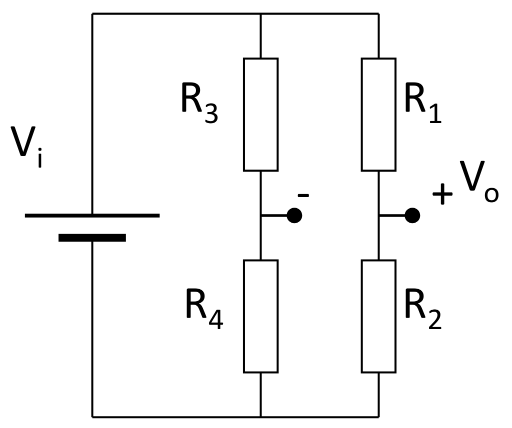
\includegraphics[width=0.74\linewidth]{strain-gauges-wheatstone-bridge-circuit-diagram}

  Wheatstone bridge equations: \\
  \(\frac{V^+}{V_i} = \frac{R_2}{R_1 + R_2}\) \\
  \(\frac{V^-}{V_i} = \frac{R_4}{R_3 + R_4}\) \\
  \(\frac{V_0}{V_i} = \frac{R_2}{R_1 + R_2} - \frac{R_4}{R_3 + R_4}\)

  Bridge balance condition: \\
  \(V_o = 0 \quad \Leftrightarrow \quad R_1 R_4 = R_2 R_3\)

  1st order approximation: \\
  \(\frac{dV_o}{V_i} = \frac{1}{4} \left(\frac{dR_2}{R_2} - \frac{dR_1}{R_1} + \frac{dR_3}{R_3} - \frac{dR_4}{R_4} \right)\)

  Wheatstone bridge strain equations: \\
  \(S_1 = S^a + S^b + S^T\) \\
  \(S_2 = S^a - S^b + S^T\)

  \subsection{Determine the sum of strains}
  \(\Diamond\) A strain gauge connected from the positive terminal of the battery (+) to negative terminal of the output (-) connection is added. \\
  \(\Diamond\) A strain gauge connected from the positive terminal of the battery (+) to positive terminal of the output (+) connection is subtracted.




  \section{Maths}

  \subsection{Derivatives}

  Chain rule: \\
  \(\frac{dz}{dx} = \frac{dz}{dy} \cdot \frac{dy}{dx}\)

  Product rule: \\
  \(\frac{d}{dx} (u \cdot v) = \frac{du}{dx} \cdot v + u \cdot \frac{dv}{dx}\)

  Quotient rule: \\
  \(\frac{d}{dx} \left(\frac{f(x)}{g(x)} \right) = \frac{f'(x) g(x) - f(x) g'(x)}{g(x)^2}\)

  Standard derivatives: \\
  \(\frac{d}{dx} \left(\sin x \right) = \cos x\) \\
  \(\frac{d}{dx} \left(\cos x \right) = - \sin x\) \\
  \(\frac{d}{dx} \left(\arcsin x \right) = \frac{1}{\sqrt{1 - x^2}}\) \\
  \(\frac{d}{dx} \left(\arccos x \right) = - \frac{1}{\sqrt{1 - x^2}}\) \\
  \(\frac{d}{dx} \left(\arctan x \right) = \frac{1}{1 + x^2}\) \\
  \(\frac{d}{dx} \left(\csc x \right) = - \csc x \cot x\) \\
  \(\frac{d}{dx} \left(\sec x \right) = \sec x \tan x\)


  \subsection{Integrals}
  \(\int \sin x \, dx = - \cos x\) \\
  \(\int \cos x \, dx = \sin x\) \\
  \(\int \frac{1}{x^2 + a^2} \, dx = \frac{1}{a} \arctan \left(\frac{x}{a} \right)\) \\
  \(\int \frac{1}{\sqrt{a^2 - x^2}} \, dx = \arcsin \left(\frac{x}{a} \right)\) \\
  \(\int \frac{1}{x^2 - a^2} \, dx = \frac{1}{2a} \ln \left|\frac{x - a}{x + a} \right|\) \\
  \(\int \frac{1}{a^2 - x^2} \, dx = \frac{1}{2a} \ln \left|\frac{a + x}{a - x} \right|\) \\
  \(\int \frac{1}{\sqrt{x^2 - a^2}} \, dx = \ln \left|\sqrt{x^2 - a^2} + x \right|\) \\
  \(\int \tan x \, dx = \ln |\sec x|\) \\
  \(\int \cot x \, dx = \ln |\sin x|\) \\
  \(\int \csc x \, dx = - \ln |\csc x + \cot x|\) \\
  \(\int \sec x \, dx = - \ln |\sec x + \tan x|\)

  Integration by parts: \\
  \(\int u \, dv = uv - \int v \, du\)


  \subsection{Trigonometric identities}

  Quotient identities: \\
  \(\tan \theta = \frac{\sin \theta}{\cos \theta}\) \\
  \(\cot \theta = \frac{\cos \theta}{\sin \theta}\)

  Reciprocal identities: \\
  \(\sin \theta = \frac{1}{\csc \theta}\) \\
  \(\csc \theta = \frac{1}{\sin \theta}\) \\
  \(\cos \theta = \frac{1}{\sec \theta}\) \\
  \(\sec \theta = \frac{1}{\cos \theta}\) \\
  \(\tan \theta = \frac{1}{\cot \theta}\) \\
  \(\cot \theta = \frac{1}{\tan \theta}\)

  Pythagorean identities: \\
  \(\sin^2 \theta + \cos^2 \theta = 1\) \\
  \(\sec^2 \theta - \tan^2 \theta = 1\) \\
  \(\csc^2 \theta - \cot^2 \theta = 1\)

  Even/odd identities: \\
  \(\sin(- \theta) = - \sin \theta\) \\
  \(\cos (- \theta) = \cos \theta\) \\
  \(\tan(- \theta) = - \tan \theta\) \\
  \(\cot (- \theta) = - \cot \theta\) \\
  \(\csc(- \theta) = - \csc \theta\) \\
  \(\sec (- \theta) = \sec \theta\)

  Co-function identities: \\
  \(\sin \left(\frac{\pi}{2} - \theta \right) = \cos \theta\) \\
  \(\cos \left(\frac{\pi}{2} - \theta\right) = \sin \theta \) \\
  \(\tan \left(\frac{\pi}{2} - \theta \right) = \cot \theta\) \\
  \(\cot \left(\frac{\pi}{2} - \theta\right) = \tan \theta \) \\
  \(\csc \left(\frac{\pi}{2} - \theta \right) = \sec \theta\) \\
  \(\sec \left(\frac{\pi}{2} - \theta\right) = \csc \theta \) \\
  \(\frac{\pi}{2} \text{ radians} = 90^{\circ}\)

  Sum/difference identities: \\
  \(\sin (\theta \pm \phi) = \sin \theta \cos \phi \pm \cos \theta \sin \phi\) \\
  \(\cos (\theta \pm \phi) = \cos \theta \cos \phi \mp \sin \theta \sin \phi\) \\
  \(\tan (\theta \pm \phi) = \frac{\tan \theta \pm \tan \phi}{1 \mp \tan \theta \tan \phi}\)

  Double angle identities: \\
  \(\sin (2 \theta) = 2 \sin \theta \cos \theta\) \\
  \(\cos (2 \theta) = \cos^2 \theta - \sin^2 \theta\) \\
  \(\cos (2 \theta) = 2 \cos^2 \theta - 1\) \\
  \(\cos (2 \theta) = 1 - 2 \sin^2 \theta\) \\
  \(\tan (2 \theta) = \frac{2 \tan \theta}{1 - \tan^2 \theta}\)

  Half angle identities: \\
  \(\sin^2 \theta = \frac{1 - \cos (2 \theta)}{2}\) \\
  \(\cos^2 \theta = \frac{1 + \cos (2 \theta)}{2}\) \\
  \(\tan^2 \theta = \frac{1 - \cos (2 \theta)}{1 + \cos (2 \theta)}\)

  Sum to product of 2 angles: \\
  \(\sin \theta + \sin \phi = 2 \sin \left( \frac{\theta + \phi}{2} \right) \cos \left( \frac{\theta - \phi}{2} \right)\) \\
  \(\sin \theta - \sin \phi = 2 \cos \left( \frac{\theta + \phi}{2} \right) \sin \left( \frac{\theta - \phi}{2} \right)\) \\
  \(\cos \theta + \cos \phi = 2 \cos \left( \frac{\theta + \phi}{2} \right) \cos \left( \frac{\theta - \phi}{2} \right)\) \\
  \(\cos \theta - \cos \phi = - 2 \sin \left( \frac{\theta + \phi}{2} \right) \sin \left( \frac{\theta - \phi}{2} \right)\)

  Product to sum of 2 angles: \\
  \(\sin \theta \sin \phi = \frac{\cos (\theta - \phi) - \cos (\theta + \phi)}{2}\) \\
  \(\cos \theta \cos \phi = \frac{\cos (\theta - \phi) + \cos (\theta + \phi)}{2}\) \\
  \(\sin \theta \cos \phi = \frac{\sin (\theta + \phi) + \sin (\theta - \phi)}{2}\) \\
  \(\cos \theta \sin \phi = \frac{\sin (\theta + \phi) - \sin (\theta - \phi)}{2}\)

  Law of sines: \\
  \(\frac{a}{\sin A} = \frac{b}{\sin B} = \frac{c}{\sin C}\)

  Law of cosines: \\
  \(a^2 = b^2 + c^2 - 2bc \cos A\)

  Area of a triangle: \\
  \(A = \frac{1}{2} ab \sin C\)

\end{multicols*}
\end{document}
